\documentclass[a4paper,14pt]{extarticle} 
\usepackage[a4paper,top=1.5cm, bottom=1.5cm, left=2cm, right=1cm]{geometry}
%\usepackage[T2A]{fontenc}
%\usepackage[english, russian]{babel}
\usepackage{graphicx}
\DeclareGraphicsExtensions{.pdf,.png,.png}
\usepackage{fontspec}
\setmainfont{Times New Roman}
\setsansfont{FreeSans}
\setmonofont{FreeMono}
\renewcommand{\baselinestretch}{1.5}
\usepackage{polyglossia}
\setdefaultlanguage{russian}
\setotherlanguages{english,russian}
\usepackage{setspace}
\usepackage[many]{tcolorbox}
\usepackage{listings}
\usepackage{multicol}
\usepackage{xcolor}
\usepackage{pdfpages}

\definecolor{codegreen}{rgb}{0,0.6,0}
\definecolor{codegray}{rgb}{0.5,0.5,0.5}
\definecolor{codepurple}{rgb}{0.58,0,0.82}
\definecolor{backcolour}{rgb}{0.95,0.95,0.92}

\lstdefinestyle{mystyle}{
    backgroundcolor=\color{backcolour},   
    keywordstyle=\color{magenta},
    numberstyle=\tiny\color{codegray},
    stringstyle=\color{codepurple},
    basicstyle=\ttfamily\footnotesize,
    breakatwhitespace=false,         
    breaklines=true,                 
    captionpos=b,                    
    keepspaces=true,                 
    numbers=left,                    
    numbersep=5pt,                  
    showspaces=false,                
    showstringspaces=false,
    showtabs=false,                  
    tabsize=2
}

\lstset{style=mystyle}

\begin{document}
    \begin{center}
        \thispagestyle{empty}
        \begin{singlespace}
        МИНИСТЕРСТВО ЦИФРОВОГО РАЗВИТИЯ, СВЯЗИ И МАССОВЫХ КОММУНИКАЦИЙ РОССИЙСКОЙ ФЕДЕРАЦИИ

        ФЕДЕРАЛЬНОЕ ГОСУДАРСТВЕННОЕ БЮДЖЕТНОЕ ОБРАЗОВАТЕЛЬНОЕ

        УЧРЕЖДЕНИЕ ВЫСШЕГО ОБРАЗОВАНИЯ

        «САНКТ-ПЕТЕРБУРГСКИЙ ГОСУДАРСТВЕННЫЙ УНИВЕРСИТЕТ ТЕЛЕКОММУНИКАЦИЙ ИМ. ПРОФ. М.А. БОНЧ-БРУЕВИЧА»

        (СПбГУТ)
        \end{singlespace}
        \vspace{-1ex}
        \rule{\textwidth}{0.4pt}
        \vspace{-5ex}

        Факультет \underline{Инфокоммуникационных сетей и систем}

        Кафедра \underline{Защищенных систем связи}
        \vspace{10ex}

        \textbf{Лабораторная работа №1}\\
        


    \end{center}
    \vspace{4ex}
    \begin{flushright}
    \parbox{10 cm}{
    \begin{flushleft}
        Выполнили студенты группы ИКТЗ-83:

        \underline{Громов А.А., Миколаени М.С., Мазеин Д.С.} \hfill 

        \footnotesize \textit{ (Ф.И.О., № группы)} \hfill \rule[-0.85ex]{0.1\textwidth}{0.6pt}
        
        \hfill \textit{(подпись)} \normalsize

        Проверил:

        \underline{Казанцев А.А.} \hfill \rule[-0.85ex]{0.1\textwidth}{0.6pt}

        (\footnotesize \textit{уч. степень, уч. звание, Ф.И.О.) \hfill (подпись)} \normalsize

    \end{flushleft}
    }
    \end{flushright}
    \begin{center}
        \vfill
        Санкт-Петербург

        2021

    \end{center}
    \newpage


    \textbf{Часть 1 - Настройка фильтрации пакетов (фаервол)}
    \begin{center}

        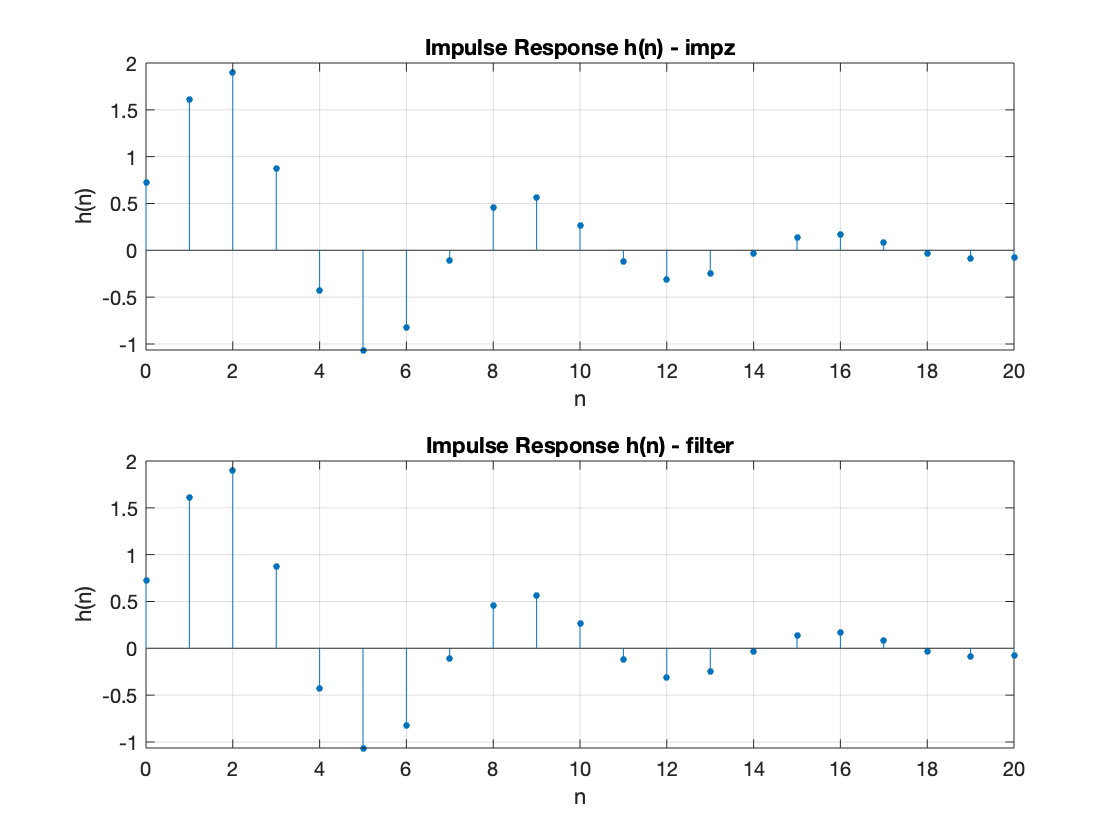
\includegraphics[scale=0.5]{pics/1.png}

        Рис. 1 Выводим список правил iptables.
        \vspace{1ex}

        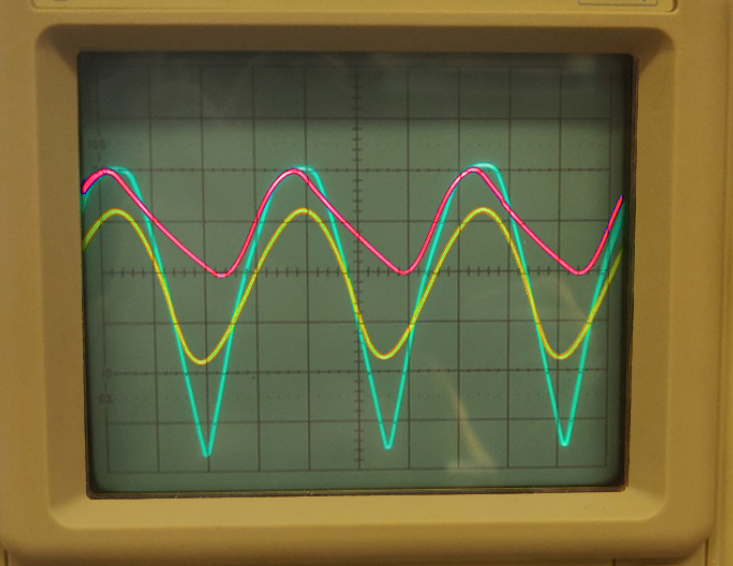
\includegraphics[scale=0.5]{pics/2.png}

        Рис. 2 Выводим список правил iptables подробнее.
        \vspace{1ex}

        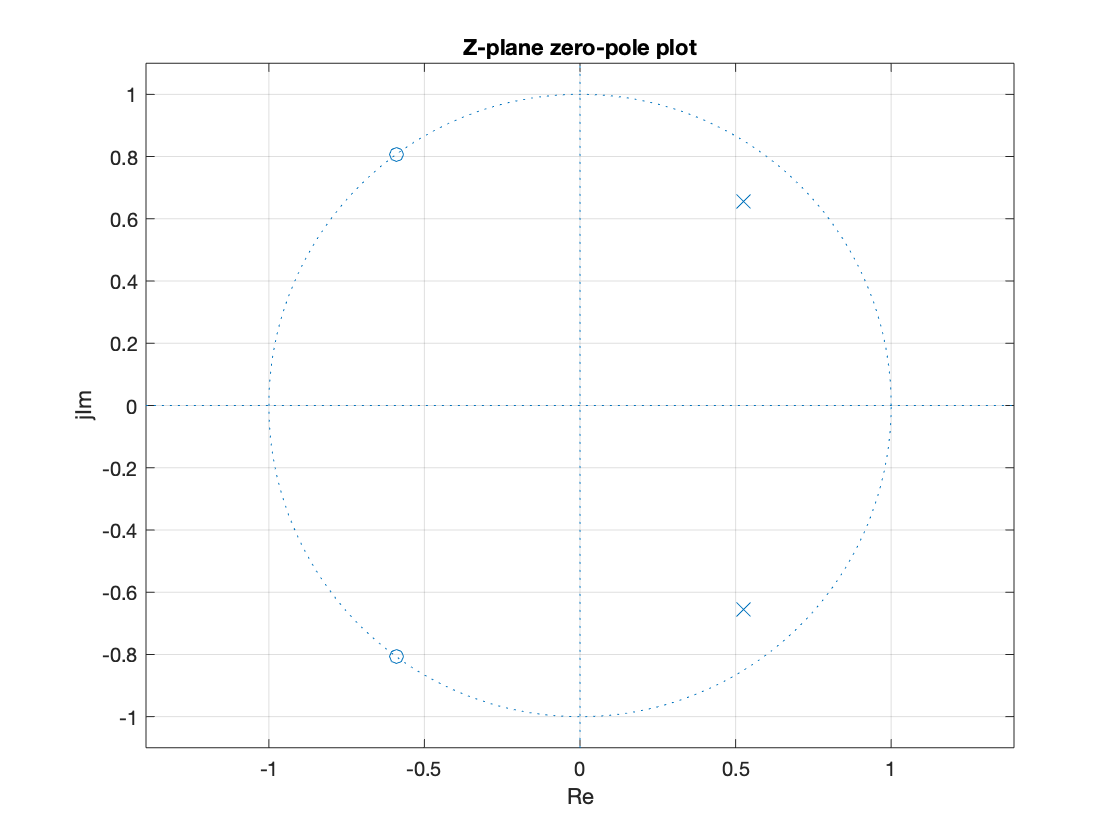
\includegraphics[scale=0.5]{pics/3.png}

        Рис. 3 Выводим список команд необходимых для активации правил и политик.
        \vspace{1ex}

        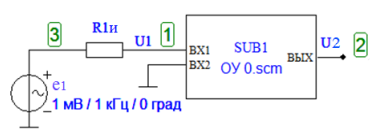
\includegraphics[scale=0.5]{pics/4.png}

        Рис. 4 Разрешаем трафик на 80 и 22 порты для tcp протокола.
        \vspace{1ex}

        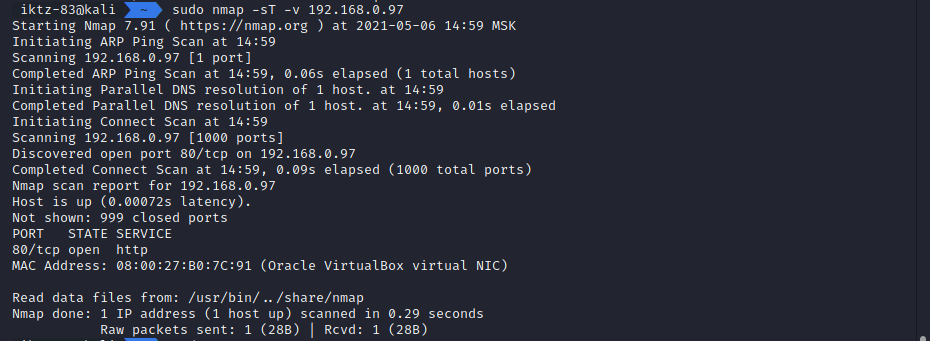
\includegraphics[scale=0.5]{pics/5.png}

        Рис. 5 Удаляем разрешение для порта 22.
        \vspace{1ex}

        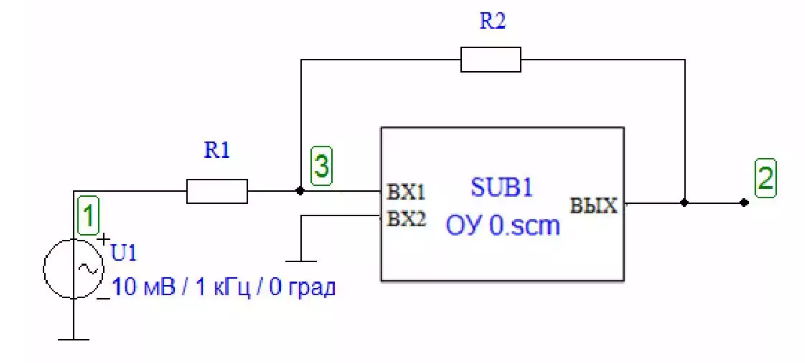
\includegraphics[scale=0.5]{pics/6.png}

        Рис. 6 Правило, позволяющее устанавливать исходящее соединение.  
        \vspace{1ex}

        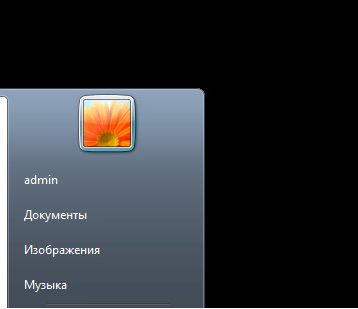
\includegraphics[scale=0.5]{pics/7.png}
        
        Рис. 7 Запрещаем все входящие и разрешаем все исходящие.
        \vspace{1ex}

        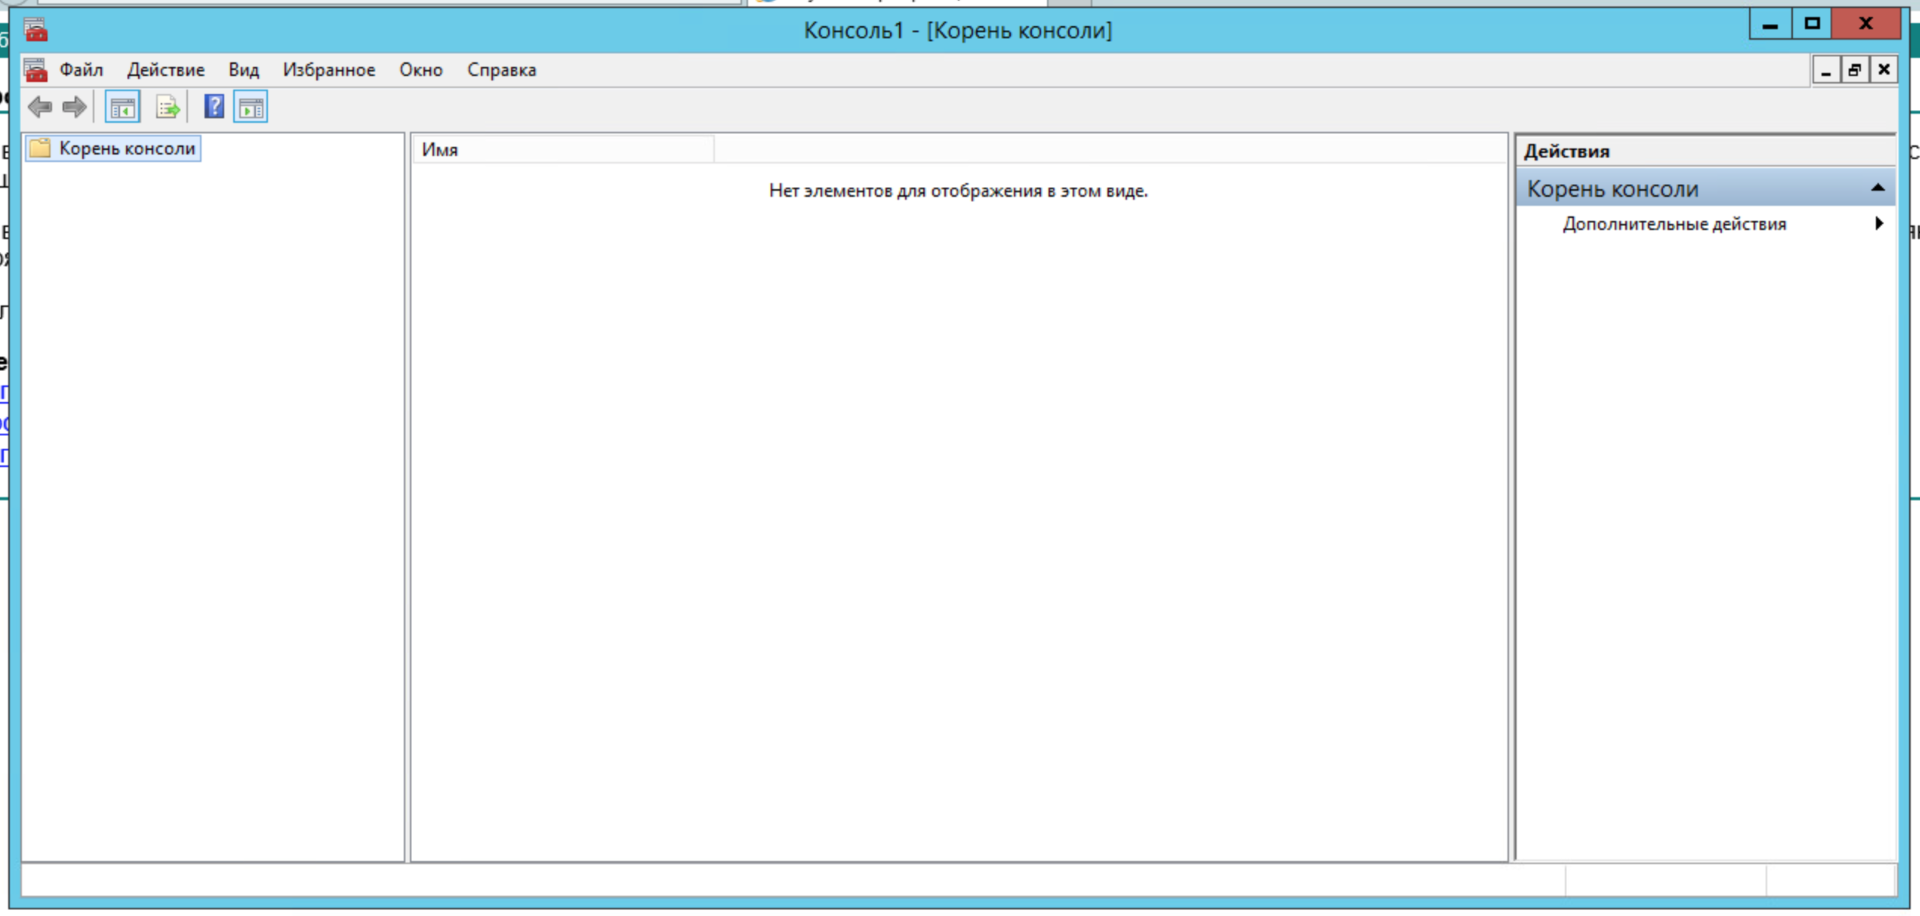
\includegraphics[scale=0.5]{pics/8.png}

        Рис. 8  Правила для блокировки наиболее распространенных атак.
        \vspace{1ex}
    \end{center}

    \newpage
    \textbf{Часть 2 - Мониторинг журналов с использованием logcheck}
    \begin{center}

        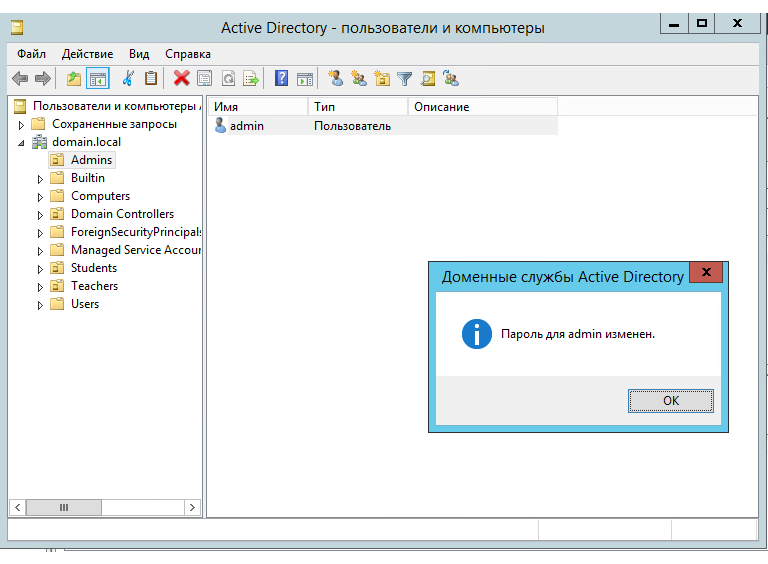
\includegraphics[scale=0.5]{pics/9.png}

        Рис. 9 logcheck успешно установлен. 
        \vspace{1ex}

        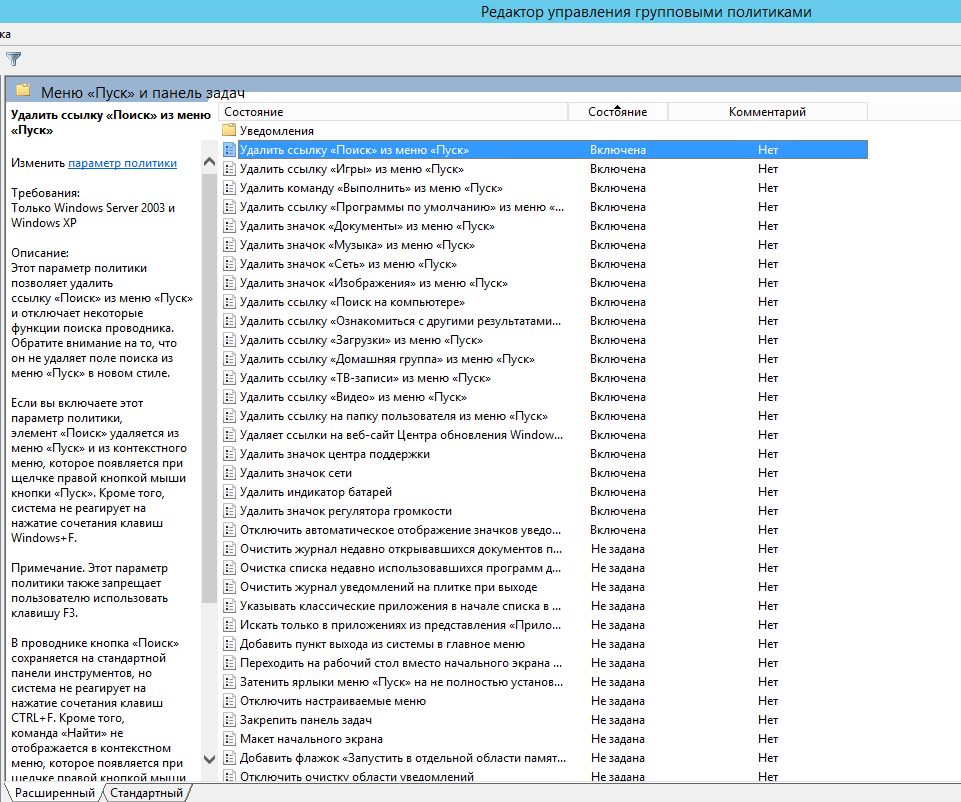
\includegraphics[scale=0.5]{pics/10.png}

        Рис. 10 Изменили REPORTLEVEL с server на paranoid.
        \vspace{1ex}

        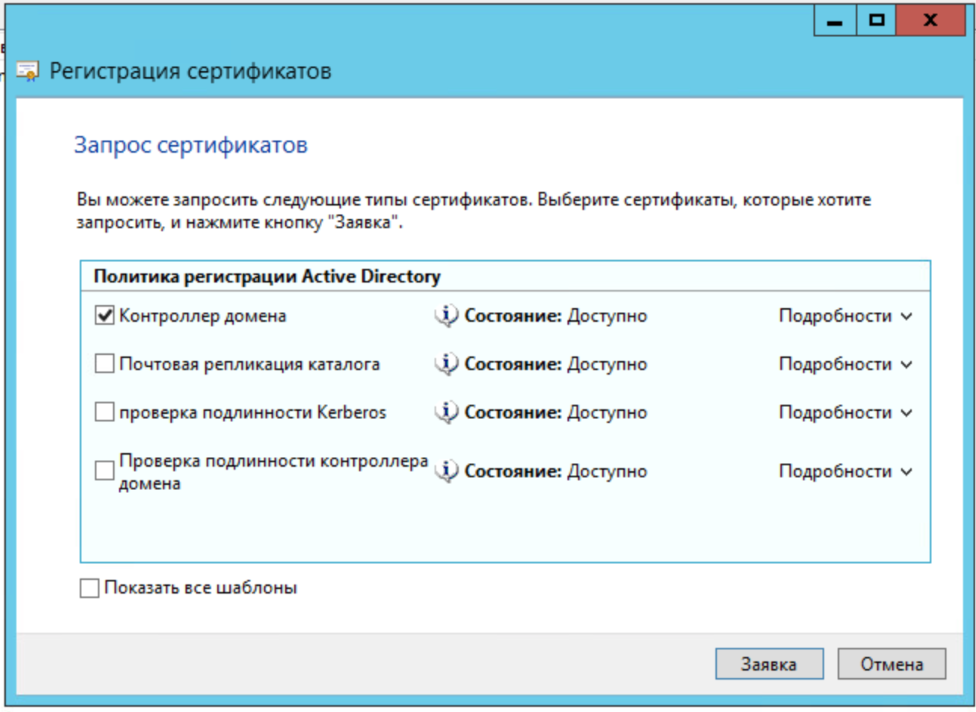
\includegraphics[scale=0.5]{pics/11.png}

        Рис. 11  Логи из файла /var/log/syslog.
        \vspace{1ex}

   \end{center}

   \textbf{Часть 3 - Установка и настройка netfilter}
   \begin{center}
       
        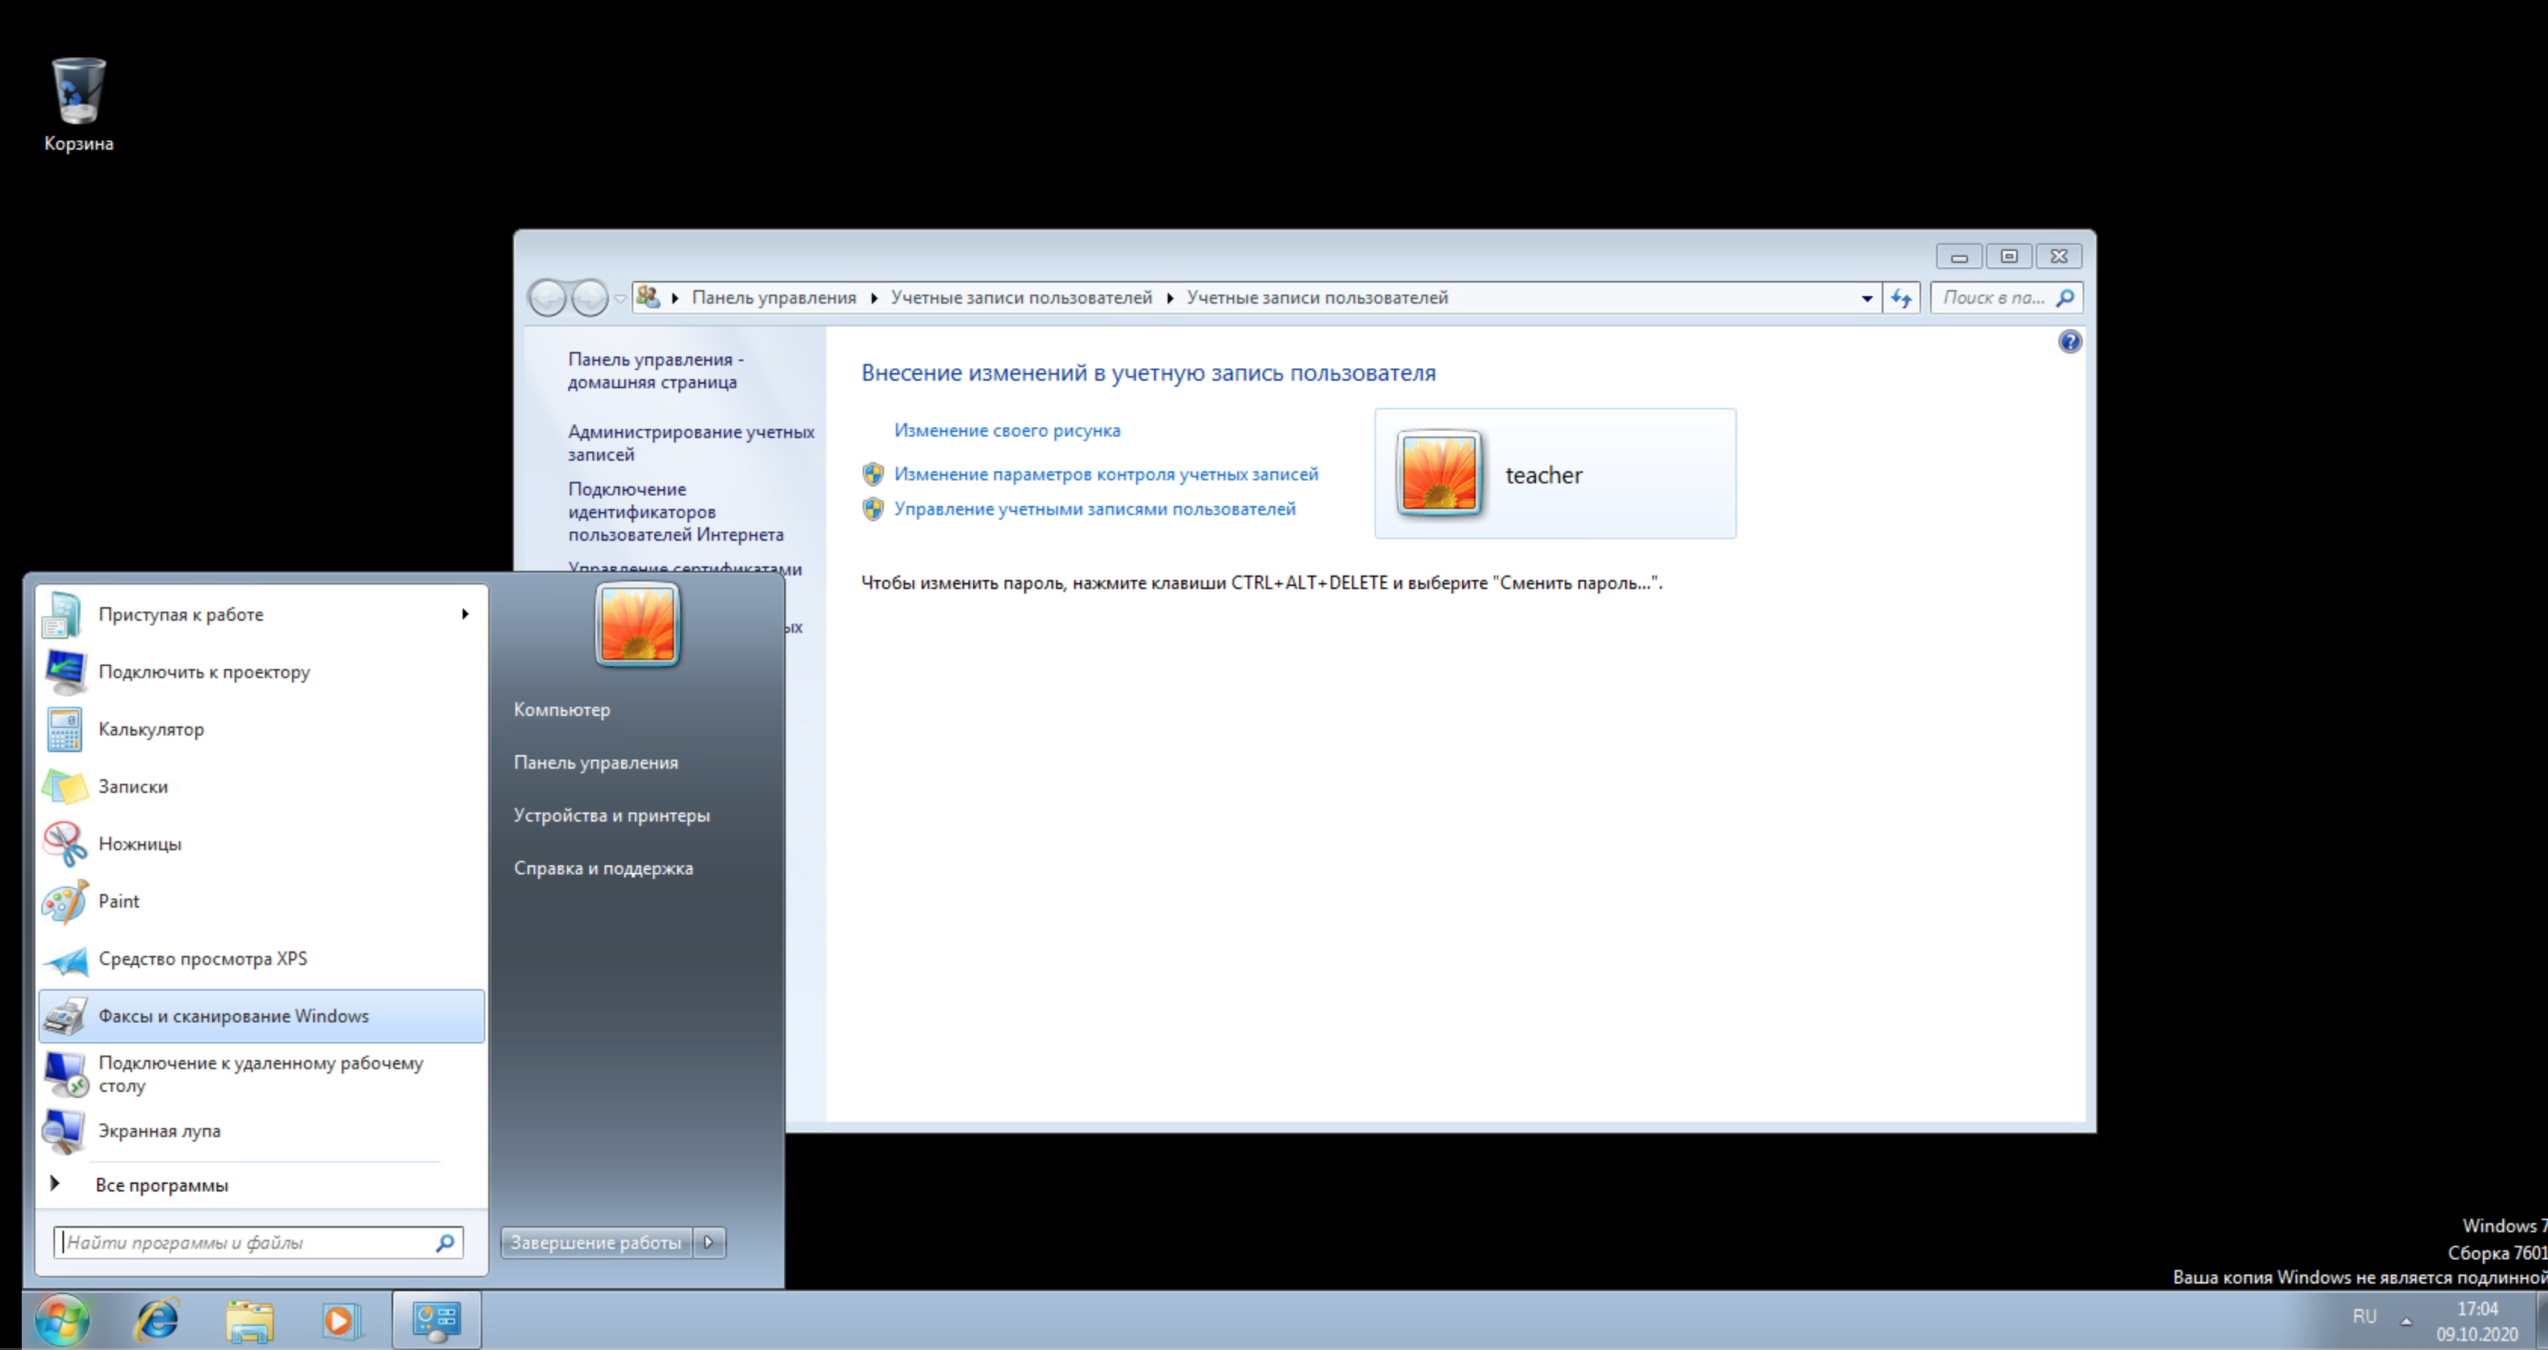
\includegraphics[scale=0.45]{pics/12.png}

        Рис. 12 Помечаем каждый пакет с помощью модуля conntrack.
        \vspace{1ex}

        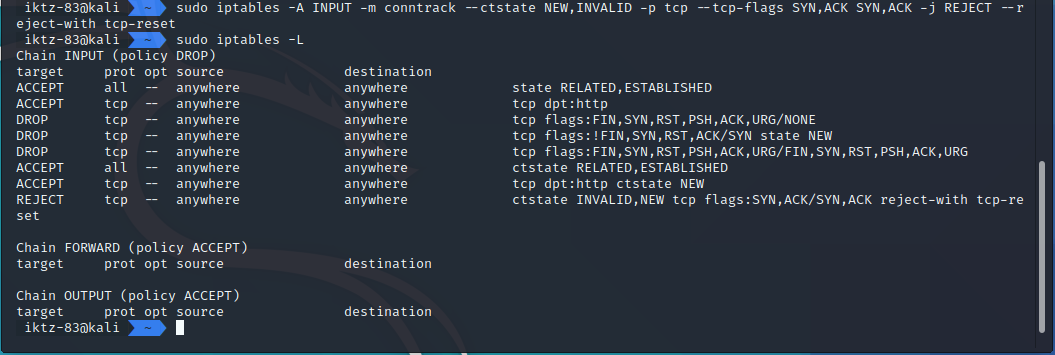
\includegraphics[scale=0.45]{pics/13.png}

        Рис. 13 Сопоставляем метки с состоянием битов.
        \vspace{1ex}

   \end{center}

   \textbf{Часть 4 - Осуществить защиту файловой системы.}
   \begin{center}
       
        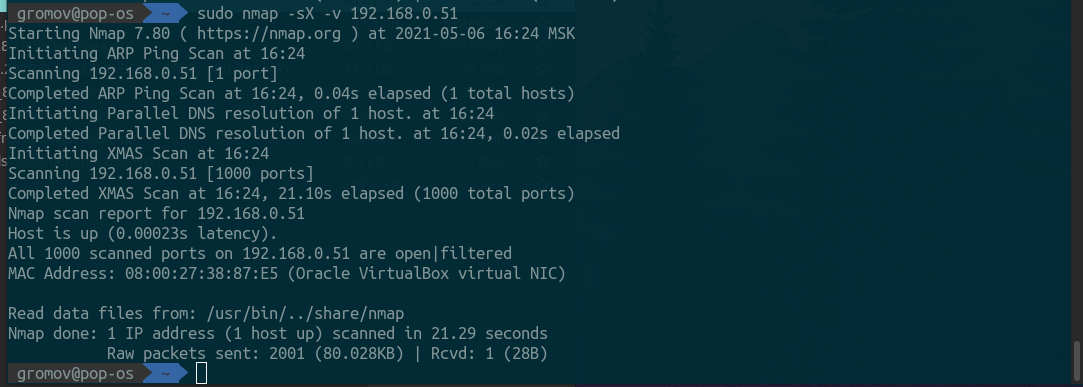
\includegraphics[scale=0.45]{pics/14.png}

        \begin{singlespace}
            Рис. 14 Подменяем внутренный ip на внешний для всех пакетов, а также разрешаем
        \vspace{1ex}
            перенаправлять пакеты между внутренними интерфейсами.
        \end{singlespace}

        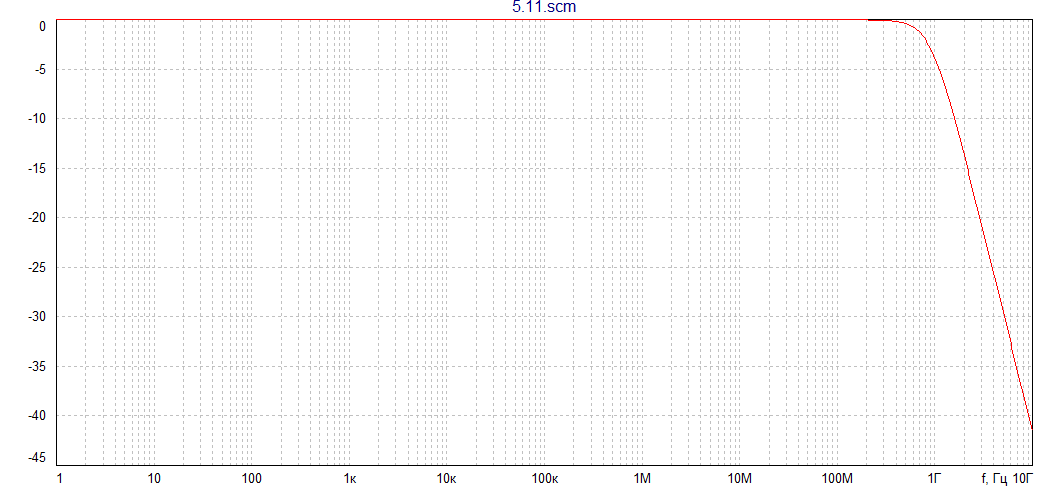
\includegraphics[scale=0.45]{pics/15.png}

        Рис. 15 Устанавливаем пакет iptables-persistent.
        \vspace{1ex}

   \end{center}

   \textbf{Часть 6 - Установка LOIC на Kali Linux.}
   \begin{center}
        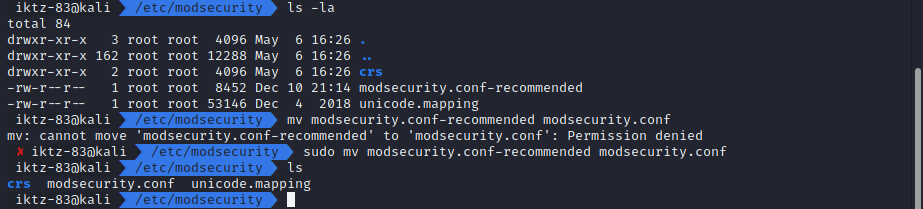
\includegraphics[scale=0.45]{pics/16.png}

        Рис. 16 Скачиваем git-core.
        \vspace{1ex}

        
\includegraphics[scale=0.45]{pics/17.png}

        Рис. 17 Устанавливаем git-core с помощью утилиты dpkg.
        \vspace{1ex}

        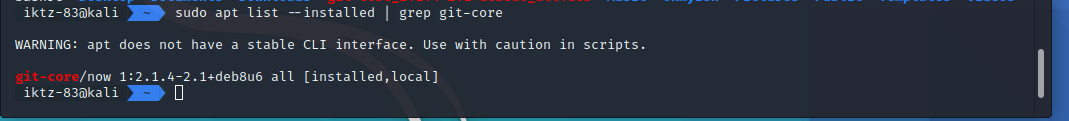
\includegraphics[scale=0.45]{pics/18.png}

        Рис. 18 Проверям установился ли пакет git-core.
        \vspace{1ex}

        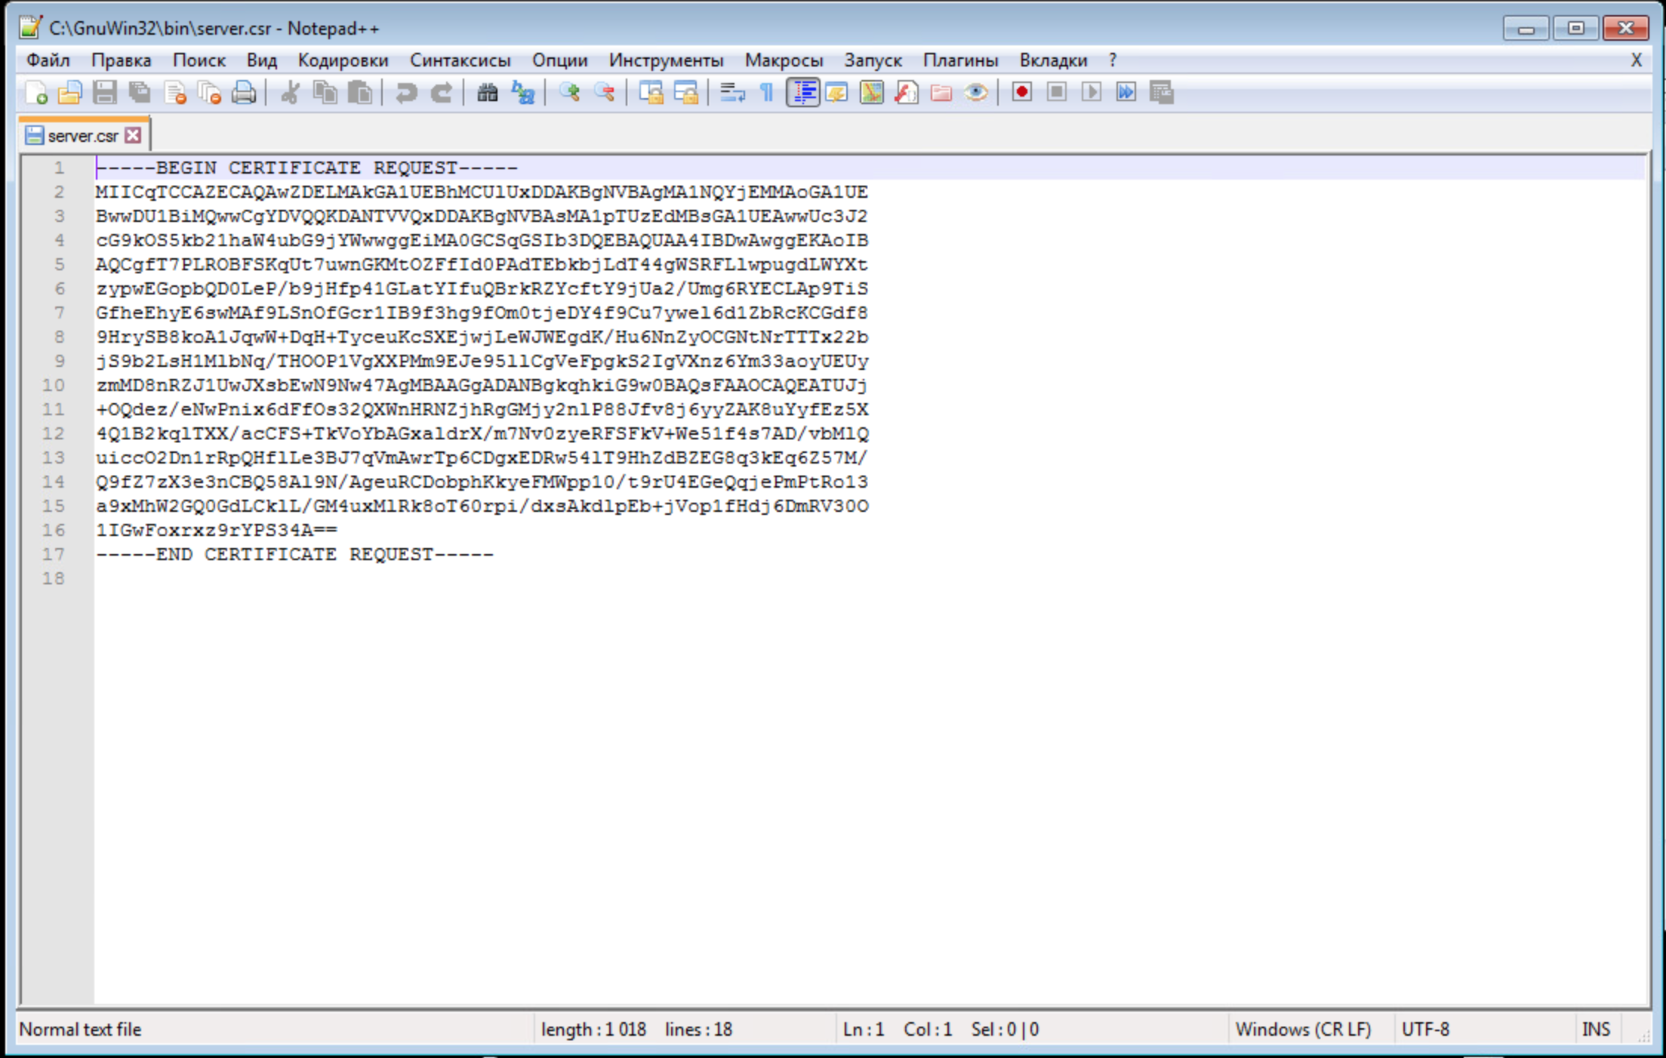
\includegraphics[scale=0.45]{pics/19.png}

        Рис. 19 Команда для установки MonoDevelop.
        \vspace{1ex}

        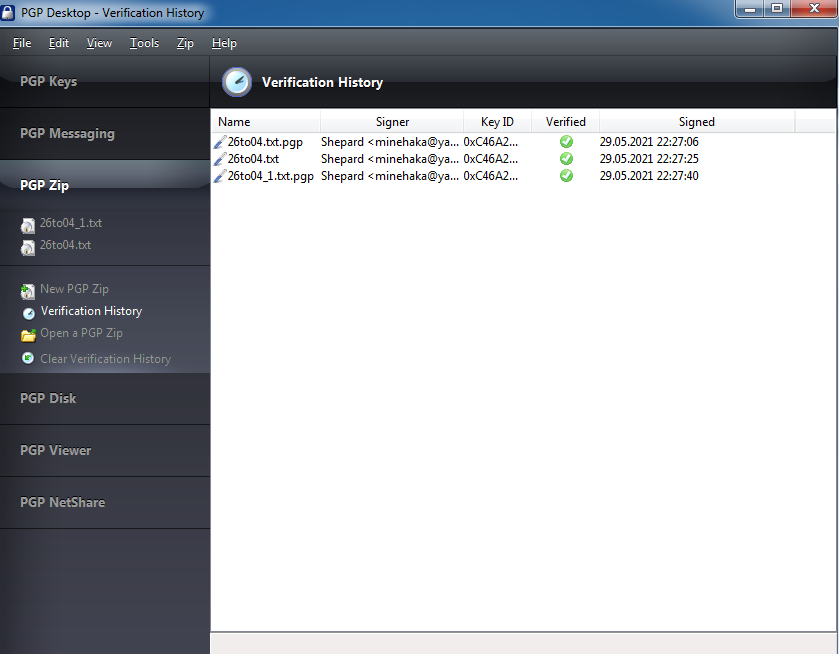
\includegraphics[scale=0.45]{pics/20.png}

        Рис. 20 Команда для установки MonoDevelop.
        \vspace{1ex}

        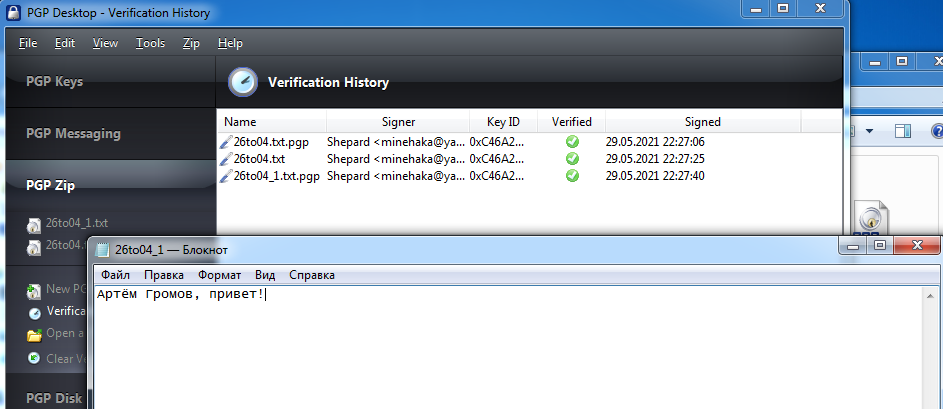
\includegraphics[scale=0.4]{pics/21.png}

        Рис. 21 Команда для установки MonoDevelop.
        \vspace{1ex}

        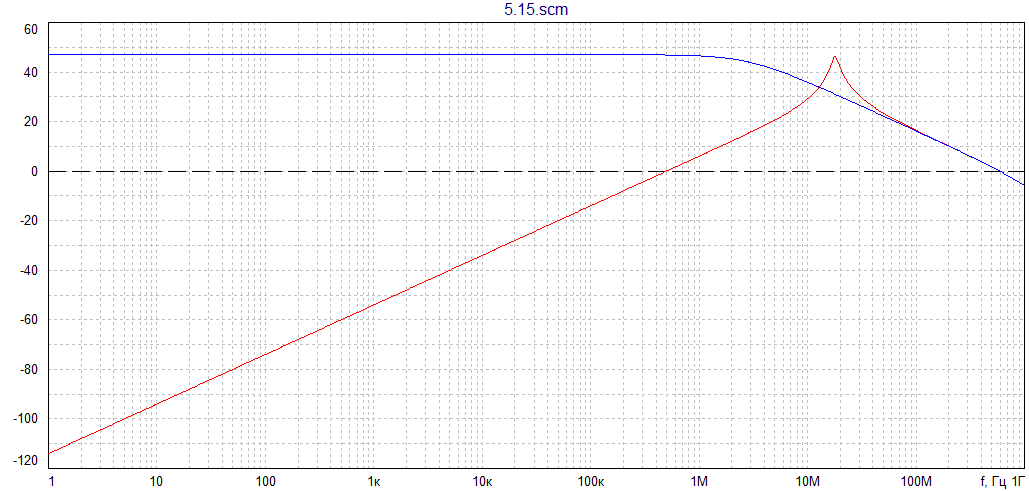
\includegraphics[scale=0.26]{pics/22.png}

        Рис. 22 Интерфейс программы MonoDevelop.
        \vspace{1ex}

        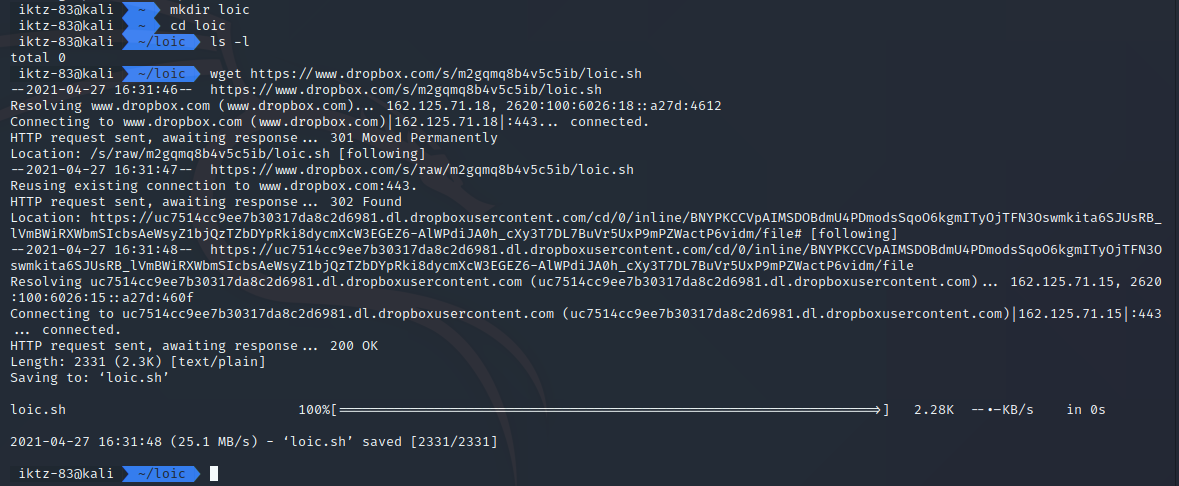
\includegraphics[scale=0.42]{pics/23.png}

        Рис. 23 Создаем папку и скачиваем скрипт для установки loic.
        \vspace{1ex}

        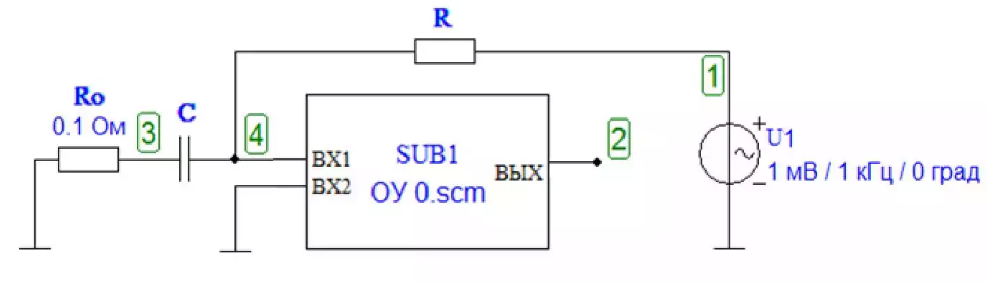
\includegraphics[scale=0.4]{pics/24.png}

        Рис. 24 Делаем скрипт исполняемым файлом.
        \vspace{1ex}

        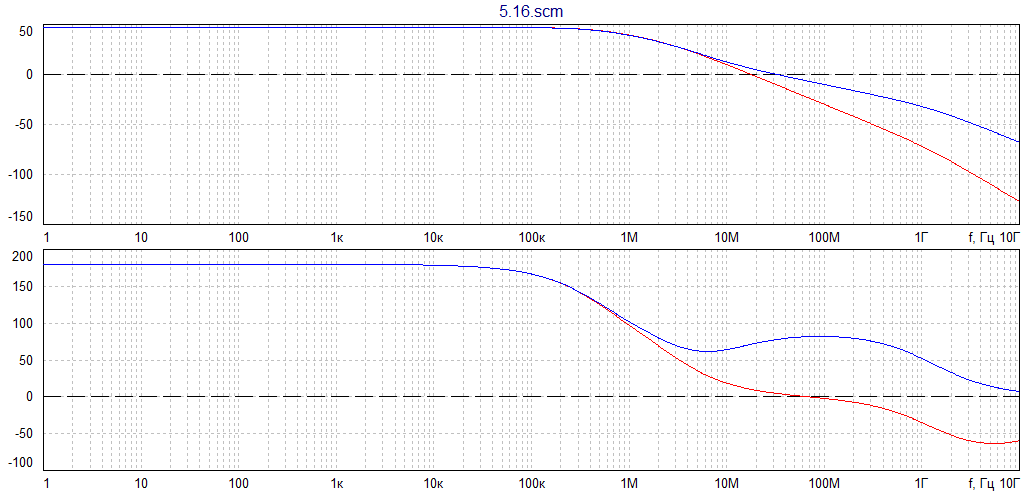
\includegraphics[scale=0.4]{pics/25.png}

        Рис. 25 Правим скрипт.
        \vspace{1ex}

        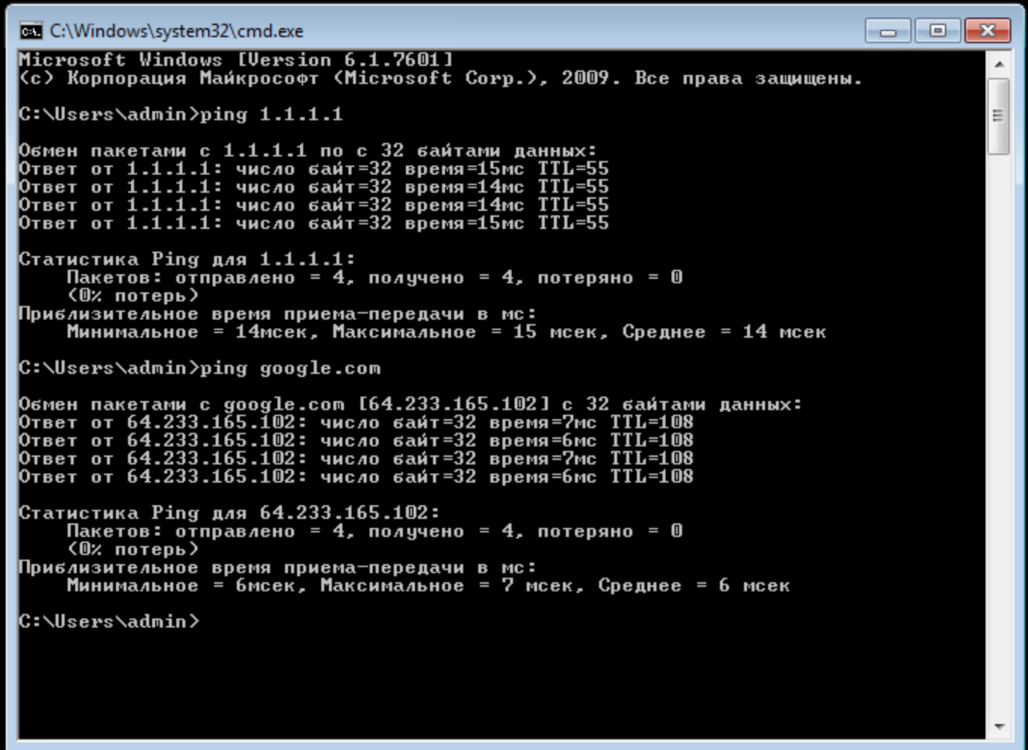
\includegraphics[scale=0.4]{pics/26.png}

        Рис. 26 Запускаем установку loic.
        \vspace{1ex}

        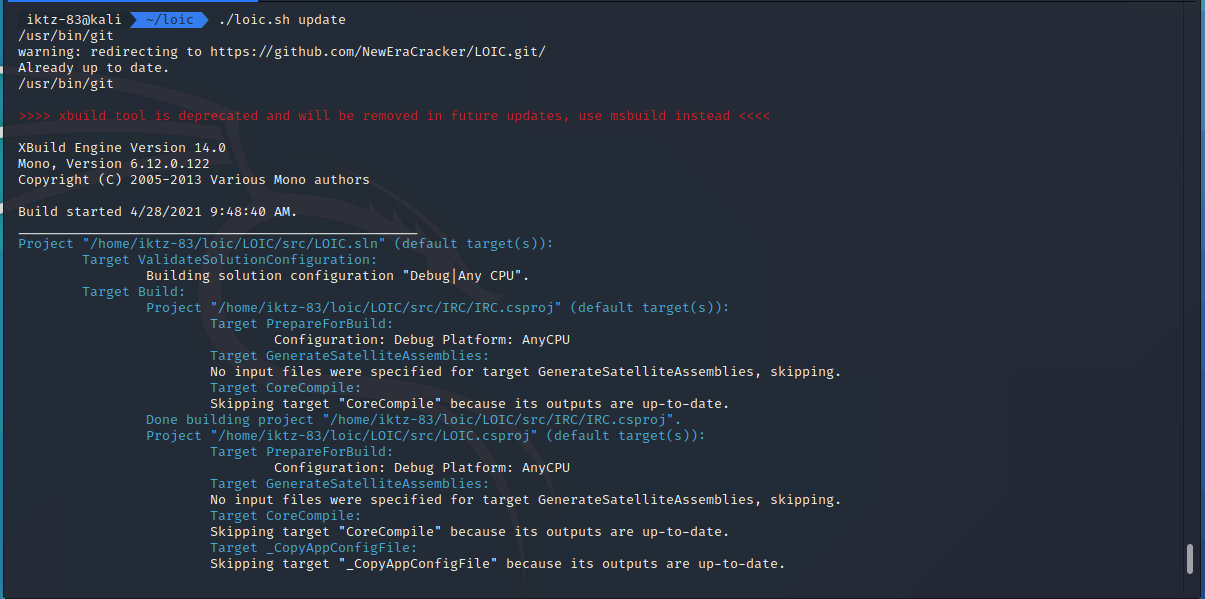
\includegraphics[scale=0.4]{pics/27.png}

        Рис. 27 Обновляем.
        \vspace{1ex}

        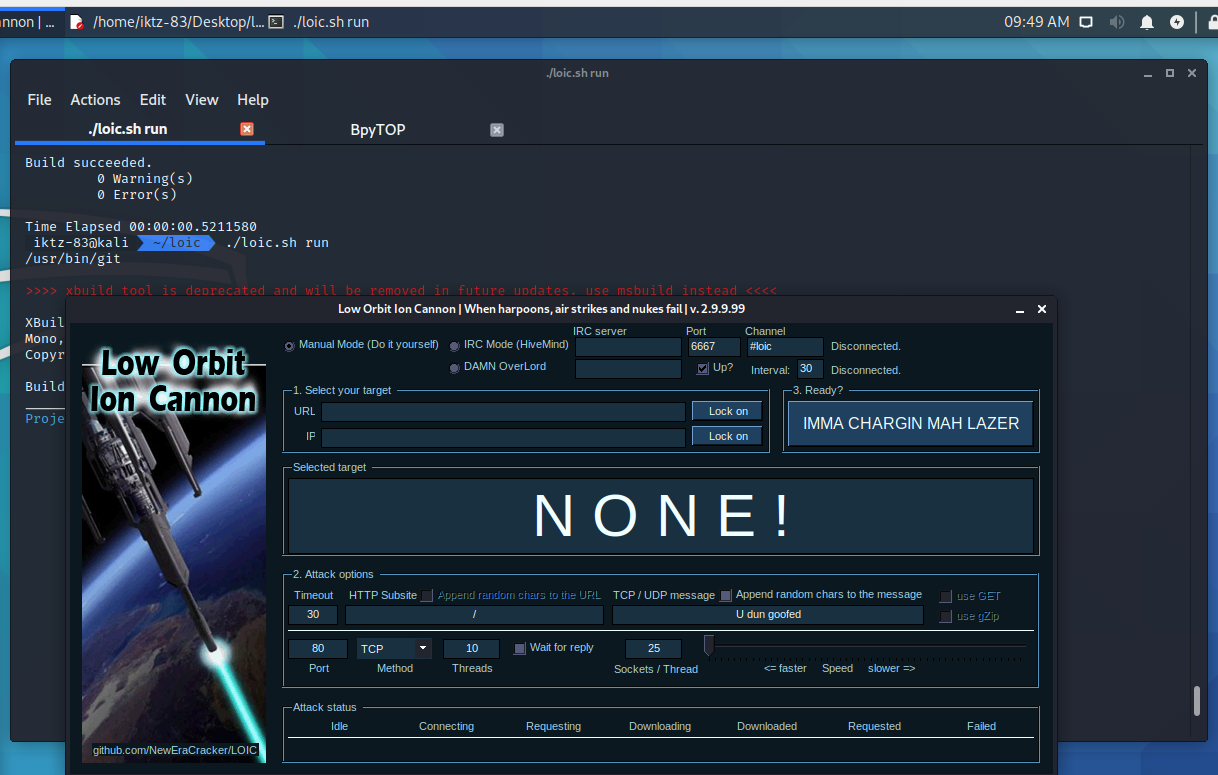
\includegraphics[scale=0.35]{pics/28.png}

        Рис. 28 Программа loic установленна, и запущена. 
        \vspace{1ex}

    \end{center}
    
    \textbf{Часть 7 - Установка Wifi\_Jammer на Kali Linux.}
    \begin{center}
        
        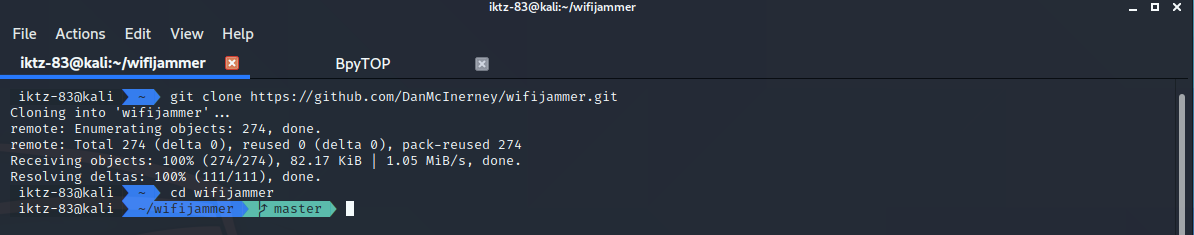
\includegraphics[scale=0.4]{pics/29.png}

        Рис. 29 Клонируем из репозитория на github wifijammer.git.
        \vspace{1ex}

        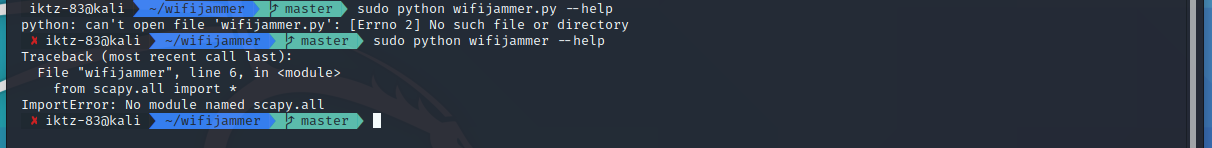
\includegraphics[scale=0.4]{pics/30.png}

        Рис. 30 Убеждаемся, что у нас не установелна библиотека scapy, для python 2.
        \vspace{1ex}

        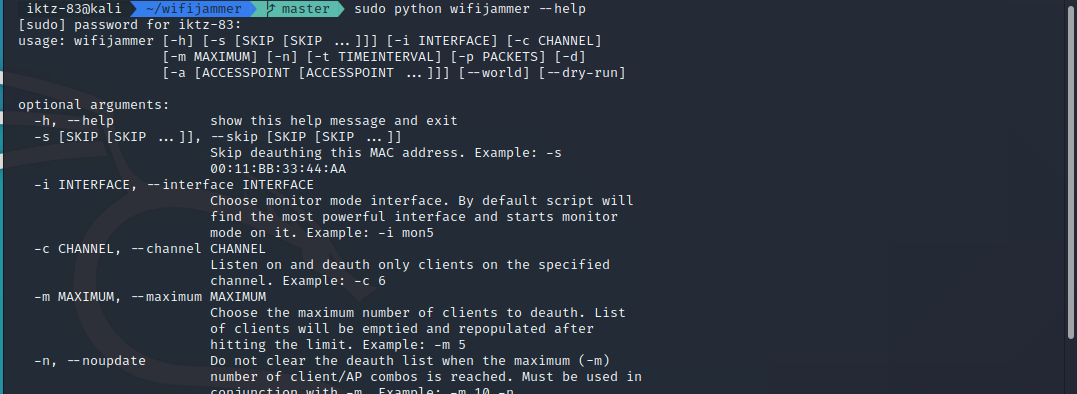
\includegraphics[scale=0.4]{pics/31.png}

        Рис. 31 wifijammer работает, после установки недостающего пакета.
        \vspace{1ex}

    \end{center}

    \textbf{Часть 8 - Использование SQLMAP на Kali Linux: взлом веб-сайтов и
баз данных через SQL-инъекции}
    \begin{center}
        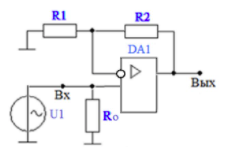
\includegraphics[scale=0.4]{pics/32.png}

        Рис. 32 Производим SQL-инъекцию со стандартным поведением.
        \vspace{1ex}

        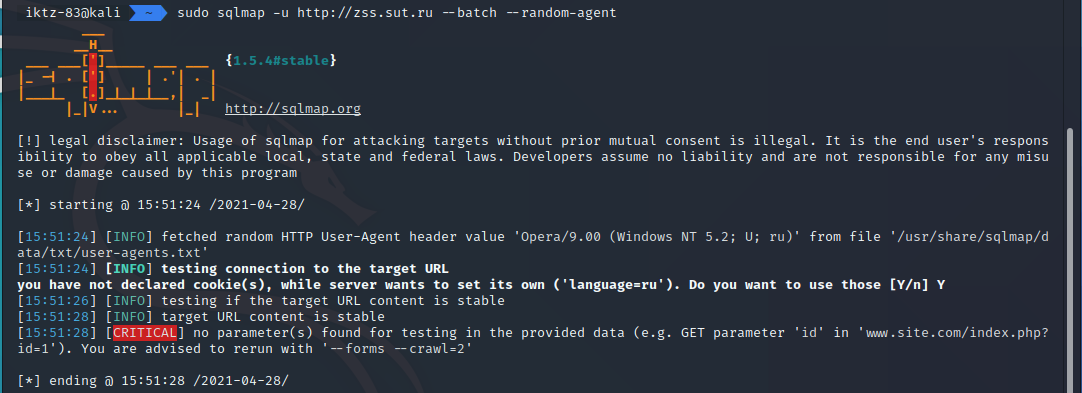
\includegraphics[scale=0.4]{pics/33.png}

        \begin{singlespace}
            Рис. 33 Производим SQL-инъекцию со стандартным поведением и случайным user-agent. 
        \vspace{1ex}
        \end{singlespace}

    \end{center}

    \textbf{Часть 9 - Crunch — генератор паролей. Установка и тест.}
    \begin{center}

        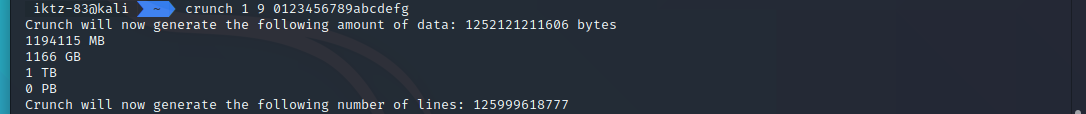
\includegraphics[scale=0.4]{pics/34.png}

        Рис. 34 Генерируем пароли от 1 до 9 цифр с использованием 0123456789abcdefg.
        \vspace{1ex}

        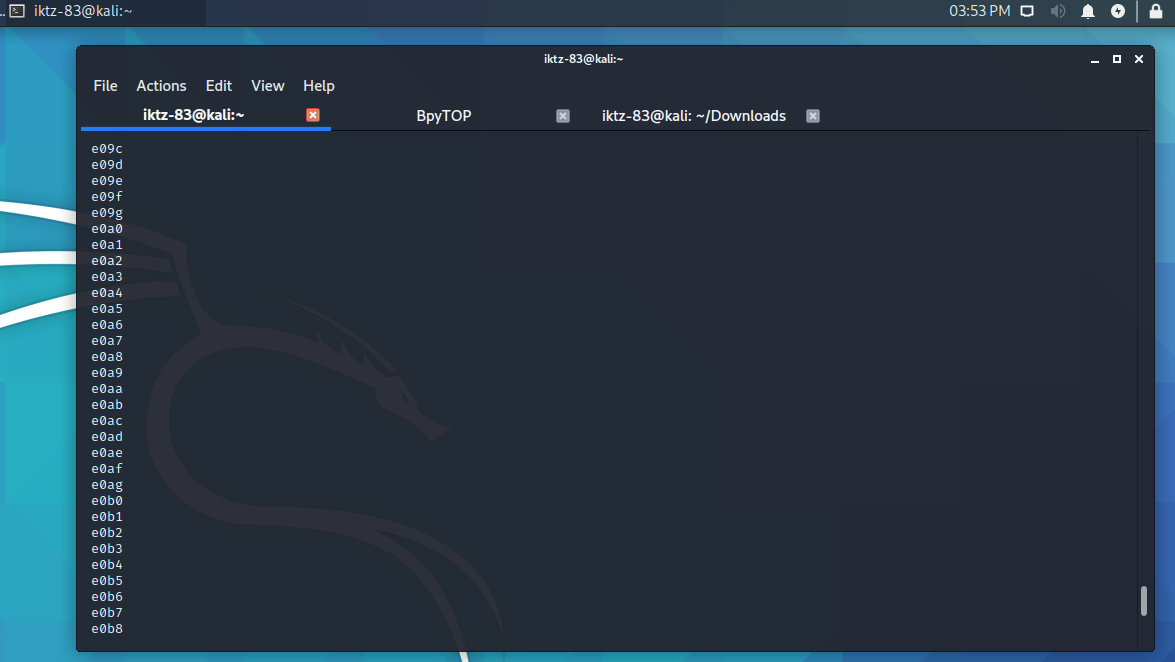
\includegraphics[scale=0.4]{pics/35.png}

        Рис. 35 Пример паролей.
        \vspace{1ex}

        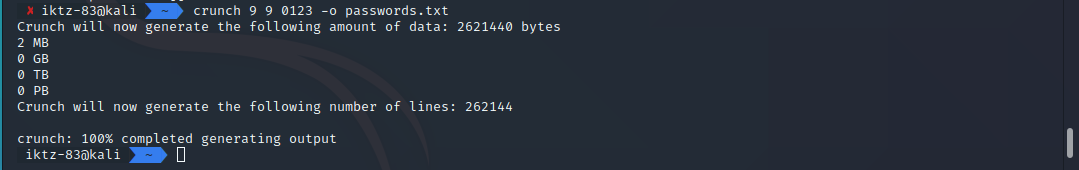
\includegraphics[scale=0.4]{pics/36.png}

        \begin{singlespace}
            Рис. 36 Генерируем пароли из 9 цифр с использованием 0123 и сохраняем их в файл passwords.txt.
        \vspace{1ex}
        \end{singlespace}

        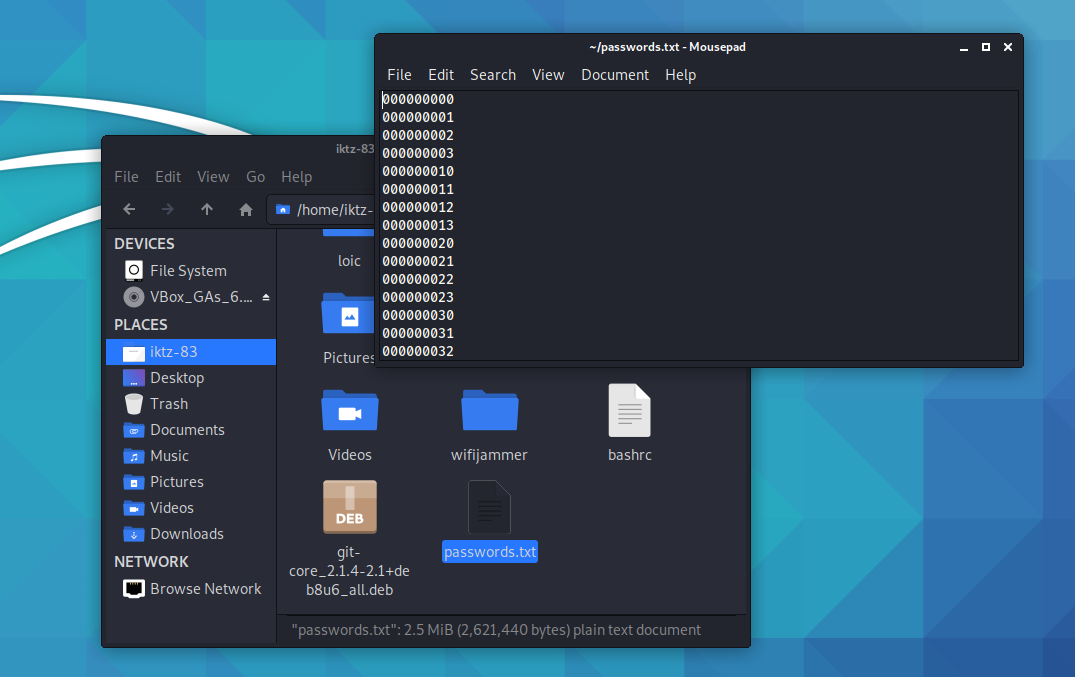
\includegraphics[scale=0.33]{pics/37.png}

        Рис. 37 Проверяем файл passwords.txt.
        \vspace{1ex}

   \end{center}

   \textbf{Вывод}

   В ходе данной лабораторной работы мы научились настраивать стандартный
   файервол linux - iptables. Также установили мониторинг журналов logcheck и \linebreak
   произвели его настройку. Установили программы MonoDevelop, Loic и wifijammer. 
   Сделали попытку совершить SQL-инъекцию на сайт zss.sut.ru, и изучили работу 
   консольной программы crunch.
\end{document}

